\documentclass{pdfmx4020}
%\documentclass{mx4020}
\usepackage{hyperref}
\usepackage{amsmath,amsthm}
% Erin's additions
\usepackage{color} 
\usepackage{graphicx}
\usepackage{float}
\usepackage{algorithm2e}
\usepackage{tikz}
\usepackage{array}
\usetikzlibrary{decorations.pathmorphing}
\usetikzlibrary{decorations.fractals}

\newtheorem*{defn}{Definition}
\newtheorem*{thm}{Theorem}
\newtheorem*{exa}{Example}
\newtheorem*{no}{Note}

\Title{Particle Swarm Optimisation for the Portfolio Selection Problem in a Function Based Environment.}
% \Title{Functional Approach }
\Author{Anthony S. Chapman}
\Year{2013--2014}
\Supervisor{Dr. Wei Pang}

\graphicspath{ {./Figures/} }

\begin{document}

% \mxfrontpage
\newfrontpage

% \begin{Summary}
% Summary....
% \end{Summary}

\begin{Abstract}
Abstract....
\end{Abstract}

\begin{Acknowledgments}
Acknowledgments....
\end{Acknowledgments}

\StartThesis

\chapter{Introduction}
  \section{Overview} % (fold)
  \label{sec:overview}
  
  % section overview (end)

  \section{Motivation} % (fold)
  \label{sec:motivation}
  % section motivation (end)

  \section{Primary Goals} % (fold)
  \label{sec:primary_goals}
  
  % section primary_goals (end)

  \section{Secondary Goals} % (fold)
  \label{sec:secondary_goals}
  
  % section secondary_goals (end)

\chapter{Background}
  In order to expand and adapt existing Particles Swarm Optimisation methods an initial background research has to be done to fully understand the concepts involved. Similarly to fully 

  \section{Particle Swarm Optimisation} % (fold)
  \label{sec:particle_swarm_optimisation}
    % Particle Swarm Optimisation (PSO) \cite{pso,pso2,pso3,pso4} is a metaheuristic inspired on the social behavior of flocks of birds when flying and on the movement of shoals of fish. A population of entities moves in the search space during the execution on the algorithm. These entities perform local interactions (with other particles as well as the environment).

    % Assuming worker bees are searching for a patch of flowers with the most pollen, also assume that the bees

    Particle swarm optimization (PSO) is a population based  stochastic optimization technique developed by Kennedy and  Eberhart in 1995, discovered through simplified social model simulation \cite{pso,pso2,pso3,pso4}. It simulates the behavior of bird flocking involving the scenario of a collection of birds randomly looking for food in a search space. None of the birds know where the food is located, they do know how far the food location is from their current position. An effective technique for the bird to find food is to adjust their velocity according to the bird which is nearest to the food. PSO was motivated from this scenario and was developed to solve complex optimization problems, where the optimum position of the fitness function is where the food is located and all the birds are the particles searching for this optimum position. 

    In the conventional PSO, the behaviour displays particles in a multidimensional space where each particles has two characteristics: a position vector and a velocity vector. Let $n$ be the number of particles in the swarm.  Then each particles $i \in n$ has the characteristics shown in \ref{eq:PSO_stuff}:
    % \begin{itemize}
    %   \item $X_i^k$ : The current position of particle i at time k.
    %   \item $V_i^k$ : The current velocity of particle i at time k. 
    %   \item $Pbest_i^k$ : The personal best position of particle i at time k. 
    %   \item $Gbest^k$ : The global best position of particle i at time k. 
    % \end{itemize}
    \begin{equation} \label{eq:PSO_stuff}
      \begin{split}
        & V_i^k \text{ : The velocity of particle i at time k.} \\
        & X_i^k \text{ : The current position of particle i at time k.} \\
        & Pbest_i^k \text{ : The personal best position of particle i at time k.} \\
        & Gbest^k \text{ : The global best position of particle i at time k.} \\
      \end{split}
    \end{equation}

    At each step, the velocity of the ith particle will be updated according to the following equation:

    \begin{equation} \label{eq:vel}
      \begin{split}
        V_{i}^{k+1} & = \omega V_{i}^{k} + c_1 r_1 \times \Big( Pbest_{i}^{k} - X_{i}^{k} \Big) + c_2 r_2 \times \Big( Gbest^{k} - X_{i}^{k} \Big) \\
        \text{where} & \\
        & V_i^{k+1} \text{ : The velocity of particle i at time k + 1.} \\
        & V_i^k \text{ : The velocity of particle i at time k.} \\
        & X_i^k \text{ : The current position of particle i at time k.} \\
        & \omega \text{ : Inertia weight parameter.} \\
        & c_1, c_2 \text{ : Acceleration coefficients.} \\
        & r_1, r_2 \text{ : Random numbers between 0 and 1.} \\
        & Pbest_i^k \text{ : The personal best position of particle i at time k.} \\
        & Gbest^k \text{ : The global best position of particle i at time k.} \\
      \end{split}
    \end{equation}

    In the updating process \ref{eq:vel} the acceleration coefficients $c_1, c_2$ and the inertia weight $\omega$ are predefined and $r_1, r_2$ are uniformly generated random numbers in the range [0,1]

    \begin{algorithm}[H] \label{eq:pso}
      \mbox{\textbf{Initialisation}} \\
      \For{i = 1,\dots,S}{
        initPosition(i) \\
        initBestLocal(i) \\
        \If{i = 1}{initBestGlobal()} 
        \If{improvedGlobal(i)}{updateGlobalBest(i)} 
        initVelocity(i)
      }
      \mbox{\textbf{Main program}} \\      
      \While{not endingCondition()}{
        \For{i - 1,\dots, S}{
          createRnd($r_1,r_2$) \\
          updateVelocity(i$,r_1,r_2$) \\
          updatePosition(i) \\
          \If{improvedLocal(i)}{updateBestLocal(i)}
          \If{improvedGlobal(i)}{updateGlobalBest(i)}
        }
      }
      \caption{PSO pseudo-code.}
    \end{algorithm}
    
    In Algorithm \ref{eq:pso} you can see the pseudo-code for a basic PSO. A step by step explanation of \ref{eq:pso}. First there is an initialisation for all the particles in the PSO, for every particle i, initPosition(i) randomly created a particle with a designated position in the search space. For the first step, initBestLocal(i) = initPosition(i) but it will be updated afterwards. Then the if function makes a first global best and if any other particles has a better global best position it will be set as the new global best. initVelocity(i) gives particles i an initial velocity which is randomly generated. 

    After the initialisation, the core of the PSO method is executed until the endingCondition() is satisfied, which can be the number of iterations or an improvement threshold. In the body of the \textit{While} loop all particles are updated. The first step is to generate random numbers used in the velocity equation \ref{eq:vel}. Then the actual velocity is updated. The next step, updatePosition(i) updates the position of a particles in the search space and checks the fitness function value for improvement or not. A the end of the \textit{for} loop, if improvedLocal(i) = True then updates the local best position and finally it's similar for updating the global best position. 

    
  % section particle_swarm_optimisation (end)

  \section{Portfolio Management} % (fold)
  \label{sec:portfolio_management}
    The money maker...
  % section portfolio_management (end)

  \section{Haskell} % (fold)
  \label{sec:haskell}
    It rules!! 
  % section haskell (end)

  % \section{Multi-objective Optimisation} % (fold)
  % \label{sec:multi_objective_optimisation}
    
  % % section multi_objective_optimisation (end)


\chapter{Related Work}
  \section{Markowitz Model} % (fold)
  \label{sec:markowitz_model}
    One of the first contributions to the portfolio problem was made by Markowitz \cite{marko1} which was later described in more detail in his book \cite{marko2}. Markowitz introduced the mean-variance model which considers the variance of the portfolio as the measure of the investor's risk under a set of assumptions. According to Markowitz, the portfolio selection problem can be expressed as an objective function subject to linear constraints. 

    Following Markowitz, the investment horizon includes a single period whereas the investment strategy is to select an optimal portfolio at the beginning of the period which will be held unchanged until the date of termination. The joint distribution of one-period security returns is assumed to be a multivariate normal distribution, which in turn follows that the distribution of the portfolio return is also normal. 

    Let $S = (S_1,S_2,S_3, \dots , S_N)$ be the set of $N$ assets where each asset $S_i$ has a rate of return represented by a variable $R_i$ with a expected return $r_i$ and each pair of assets $(S_i,S_j)$ has a covariance $\sigma_{ij}$ . The variance-covariance matrix $\sigma_{n\times n}$ contains all the covariance values, furthermore, it is a symmetric matrix and every diagonal element $\sigma_{ii}$ represents the variance of asset $S_i$. Let $\pi$ be a positive value which represents the investor's required expected return. Generally the values $r_i$ $\sigma_{ij}$ are estimated from past data and are fixed during the period of investment. 

    According to Markowitz, a portfolio is a real valued vector $X = (x_1,x_2,x_3, \dots ,x_i)$ where each variable $x_i$ represents the percentage invested in a corresponding asset $S_i$. The value $\sum\limits_{i=1}^N \sum\limits_{j=1}^N x_i x_j \sigma_{ij}$ is the variance of the portfolio and it is the measure of risk associated with the portfolio. From this, we may obtain a constrained portfolio optimisation problem: 
    \begin{equation}
      \begin{split}
        Minimise \\
        \sum\limits_{i=1}^N \sum\limits_{j=1}^N x_i x_j \sigma_{ij} \\
        Constraints:\\
        \sum\limits_{i=1}^N x_i r_i = \pi \\
        \sum\limits_{i=1}^N x_i = 1 \\
        x_i \geq 1, i \in \{1,2,\dots,N\}
      \end{split}
    \end{equation}

    Here, the objective function minimises the total variance (risk) associated with a portfolio whilst the constraints ensure that the portfolio meets the expected required return of $\pi$ and the proportions of all the assets sum to 1. The non-negative constraint means that no short-selling is allowed. 

    This framework presumes that the investor uses a quadratic utility function or that asset returns follow a multivariate normal distribution. This implies that the rate of return of a portfolio of assets can be completely explained by the expected return or variance of assets. The efficient-frontier is the set of assets which provide minimum risk for a specified level of return. Solving the Markowitz portfolio optimisation problems for different specified expected portfolio returns will give us a set which represents the efficient-frontier, it is a smooth semi-increasing curve which represents the best possible trade-off between risk and expected return, also called the set of Pareto-optimal portfolios. 

    \begin{figure}[H]
      \centering
        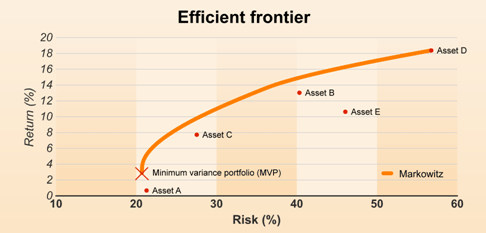
\includegraphics[width=0.9\textwidth]{efficient_frontier}
      \caption{A picture of a gull.}
      \label{efficient_frontier}
    \end{figure}

    Figure~\ref{efficient_frontier} shows an example of an efficient frontier without a risk-free asset. Each point on the line represents a portfolio which is considered to be efficient (ie no other portfolio provides higher return without more risk and similarly for risk). In~\ref{efficient_frontier} Asset A-E represent what the portfolio will be made out of. 

    Markowitz's model is subject to serous criticisms as stated in \cite{crit}, the main ones being that a measure of dispersion can be adopted as a measure of risk only if the relevant distribution is symmetric. Another problem is that the distribution of individual asset returns has a tendency to show a higher probability of being fat-tailed. In case of non-normal, non-symmetric distributions, the utility function must be quadratic \cite{crit}. 

    This criteria as should not be taken lightly since the assets' return does not follow normal distributions in real world situations \cite{non-dist}. This approach can only be used if the investor's utility function is quadratic with non-positive second derivatives or if the asset's return distribution can be fully described. Several research have indicated that that the quadratic utility function implies that beyond some level or return, marginal utility of the decision maker for wealth becomes negative \cite{crit2,crit3}. 

  % section markowitz_model (end)
  


  %------------------------------------------------------------------
  % \section{Heuristic and Metaheuristic Algorithms} % (fold)
  % \label{sec:heuristic_and_metaheuristic_algorithms}
  %   The use of heuristics is very attractive to solve real world problems. For many problems, a heuristic algorithm may be the unique way to obtain good solutions in a reasonably short space of time. Meta-heuristics, a subfield of general heuristic strategies, includes stochastic components to utilize randomised search capabilities. 

  %   In real world applications, 

  % % section heuristic_and_metaheuristic_algorithms (end)
  %------------------------------------------------------------------

  \section{Portfolio in Excel} % (fold)
  \label{sec:portfolio_in_excel}
    
  % section portfolio_in_excel (end)

  \section{Something PSO} % (fold)
  \label{sec:something_pso}
  
  % section something_pso (end)

  \section{PSO applied} % (fold)
  \label{sec:pso_applied}
  
  % section pso_applied (end)

\chapter{Problem Domain}
  
  Particle Swarm Optimisation Algorithms has already been effectively implemented to solved various optimisation problems \cite{pso_app,pso_app2,pso_app3} under variant domains such as biomedical, networks, clustering, finance, combinatorial and many more \cite{pso_app_main}. This project mainly focuses on expanding the optimisation algorithm created by Rabanal, Rodrıguez and Rubio in their paper ``A Functional Approach to Parallelize Particle Swarm Optimization'' \cite{haskellPSO} and more importantly, applying it to solve the portfolio selection problem \cite{marko2}. The optimisation algorithm has been successful by means of accuracy as well as efficiency. 

  When the difference between investing well and investing efficiently results in not gains hundreds of thousands of pounds, it becomes quite obvious that 

  at finding the maxima or minimia of given problems over specified domains, its special success is at not becoming trapped in local maxima or minimas even though the algorithm might encounter multiple of them before finding the global maxima or minima due to the concept of randomness being introduces, not only to each particle but also to the initialisation of the whole swarm itself. When evolutionary algorithms come across functions, such as $f(x)=\sum\limits_{i=1}^n -x_i sin(\sqrt{|x_i|})$ which was considered \cite{localmin} as a particularly hard function to optimise due to the number of local minima increases exponentially with the number of dimensions of the searching space, the danger might be that when it finds a certain local minima which might seem like a ``good enough'' solution, then the algorithm might converge to this false solution. Furthermore when what we're trying to optimise has local minima and global minima which differ by thousands of pounds worth of stocks when applied to financial situations it is crucial the algorithm does not get stuck in non-optimal solutions. 

  Mention more about portfolio optimisation....

  \section{Approach} % (fold)
  \label{sec:approach}

  
  % section approach (end)

\chapter{Requirements}
This section describes the requirements for this project. Table \ref{table:functionalRequirements} refers to the functional requirements from technical point of view. Section \ref{sec:non_functional} focuses on the non-functional requirements of the system. 
  \section{Functional} % (fold)
  \label{sec:functional}
  \begin{table}[ht]
    \setlength{\extrarowheight}{2.0pt}
    \begin{tabular}{|l|l|l|}
      \hline
      No. & Description & Priority \\
      \hline
      \textbf{1} & \textbf{Optimisation of Portfolio} & \\
      \hline 
      \textbf{1.1} & \textbf{PSO} & \\
      \hline 
      1.1.1 & Initialisation of particle population & High \\
      \hline 
      1.1.2 & Processing swarm optimisation & High \\
      \hline 
      1.1.3 & Updating the local and global (at each step) particle values& \\
      \hline 
      1.1.4 & Calculating an optimal solution & High \\
      \hline 
      1.1.5 & Presenting the results & High \\
      \hline 
      \textbf{1.2} & \textbf{PSO for portfolio problem } & \\
      \hline 
      1.2.1 & Minimise portfolio variance & High \\
      \hline 
      1.2.2 & Maximise portfolio expected return & Low \\
      \hline 
      1.2.3 & Use multi-objective for optimum solution & Low \\
      \hline 
      1.2.4 & Refining results output & High \\
      \hline 
      1.2.5 & Make results for readable for user & High \\
      \hline 
      \textbf{2} & \textbf{User Input} & \\
      \hline
      2.1 & Allow the user to enter the name of the data file & High \\
      \hline
      2.2 & Allow the user to change the expected portfolio return & High \\
      \hline 
      2.3 & Allow the user to select the name for the output file & Low \\
      \hline 
      2.4 & Allow the user to change the PSO particle size & Low \\
      \hline 
      2.5 & Allow the user to change the PSO iteration number & Low \\
      \hline
      \textbf{3} &\textbf{Output format} & \\
      \hline 
      3.1 & Display the results during run-time & High \\
      \hline 
      3.2 & Make results more readable for output file & High \\
      \hline
      3.3 & Store results into a separate file & High \\
      \hline
    \end{tabular}
    \caption{Functional requirements for system.}
    \label{table:functionalRequirements}
  \end{table}
  
  % section functional (end)

  \section{Non-functional} % (fold)
  \label{sec:non_functional}
    As this system is an extension on a PSO module by Fernando Rubio et. all \cite{haskellPSO}, it is crucially important to devote a considerable amount of time to testing. This is to ensure that the alterations do not affect the performance of the overall efficiency of the algorithm and quality of the optimisation.  

    The system's scalability is something not to be overlooked. As each asset in a portfolio represents one dimension in the fitness function (not to be confused with just another linear factor of the same coefficient in a function), optimising a function in, for example, 100 dimensions (100 assets) might be to much for the system to cope with. 

    Running the PSO requires setting up various parameters and thresholds for optimisation (size of the particle population, number of iterations, inertia weights and convergence coefficients). These parameters need to be optimised for the algorithm to be computationally effective and produce accurate results. 

  % section non_functional (end)

\chapter{Methodology and Technologies}
  This chapter describes the methodology used in the project for the research, design, implementation and testing. It also mentions the technologies used to achieve the goals. 
  \section{Methodology} % (fold)
  \label{sec:methodology}
  This sections is basically an extension to the project plan which had to be made during the first week of the project. An approximate guideline to follow the project was set focusing on the project deadlines. I left a few weeks for margin for error in case something takes slightly longer than planned for whatever reason. 

   -----Project timeline-----

  For this project to be successful I am planning on spending the initial weeks researching relevant literature and becoming familiar with the concepts of Particle Swarm Optimisation. This is a completely new field to me and understanding the key ideas and models will be critically important. Not only will I need to understand PSO's background I will also need to study previous implementations and applications in order to become absolutely comfortable with it. Finally, as I am planning on improving an existing algorithm, I will have to spend some time becoming familiar enough with the code so that I will be able to modify it with ease.

  The implementation stage will consist of designing the future system and the realisation of the plans. Key design decisions will have to be made during this stage and the solutions might be obtained from the analysis of previous work. 

  To complete this project test driven development will be carried out. I plan to test after every implementation or modification. This will be done to ensure that changes won't affect any previous functionality. The tests will evaluate the efficiency as well as the accuracy of my system. Given the nature of PSO's `random' initialisation,  I want to make sure that the results are consistent. 

  The writing of this result will be flexible, the sections will be written as needed or when the section arises naturally throughout the project. 

  % section methodology (end)

  \section{Technology} % (fold)
  \label{sec:technology}

    \subsection{Haskell} % (fold)
    \label{sub:haskell}
      Coming from a strong mathematical background I find functional languages easier to understand. Also one huge advantage of pure functional languages is that the absence of side-effects allow them to offer a clear semantic framework to analyse the correctness of programs. 

      As Haskell is the functional language I am more familiar with, I didn't see the point in learning a new language as it would only restrict my project process, so Haskell was a clear winner. 

      There are other PSO implementations in other languages such as C and Ruby but as already mentioned, Haskell is my preferred language. 

    % subsection haskell (end)
    \subsection{Operating System} % (fold)
    \label{sub:operating_system}
      As Haskell is platform independent (in the sense that it can be compiled in Windows, Linux or Mac) I have chosen to use Ubuntu 12.04 as it is my preferred OS and I feel the most comfortable with it. In addition, I wouldn't be affected in the about of software needed for the project as it is provided for all three OSs already mentioned. 

      The work was carried out on my personal laptop (Intel CORE$^{TM}$ i3 @ 2.6GHZ,4Gb RAM). If required due to any reasons, the university provide classroom PCs (Intel CORE$^{TM}$ i3-2100 CPU @3.10 GHz, 3 Gb RAM) although I have faith that my own machine will be reliable enough for me not to have to change machines. 
      Sublime Text 2 was chosen as the IDE for the project. It has many useful functions \cite{sublime} and similarly for the choice of OS, I am happy with this editor.
    % subsection operating_system (end)
  
  % section technology (end)

\chapter{System Design and Architecture}

  \section{Original PSO Implementation} % (fold)
  \label{sec:original_pso_implementation}

    \subsection{Initialisation} % (fold)
    \label{sub:initialisation}
    
    % subsection initialisation (end)
    \subsection{Optimisation} % (fold)
    \label{sub:optimisation}
    
    % subsection optimisation (end)
    \subsection{Termination} % (fold)
    \label{sub:termination}
    
    % subsection termination (end)
  % section original_pso_implementation (end)

  \section{Expansion for Portfolio Optimisation} % (fold)
  \label{sec:expansion_for_portfolio_optimisation}

    \subsection{Interface and User Input} % (fold)
    \label{sub:interface_and_user_input}
    
    % subsection interface_and_user_input (end)
    \subsection{Optimisation} % (fold)
    \label{sub:optimisation}
    
    % subsection optimisation (end)
    \subsection{Termination} % (fold)
    \label{sub:termination}
    
    % subsection termination (end)
    \subsection{Fitness Function} % (fold)
    \label{sub:fitness_function}
    
    % subsection fitness_function (end)
    \subsection{Presenting the Results} % (fold)
    \label{sub:presenting_the_results}
    
    % subsection presenting_the_results (end)
  % section expansion_for_portfolio_optimisation (end)



\chapter{Experimentation and Testing}

  \section{Constriction Factors} % (fold)
  \label{sec:constriction_factors}
    Maurice Clerc in his study on stability and convergence of PSO \cite{constriction_factor} has introduced a constriction factor. Clerc indicates that the use of a constriction factor may be necessary to insure convergence of the PSO for certain fitness functions.

    In order to ensure convergence of the PSO, the velocity of the constriction factor based approach can be expressed as follows:

    \begin{equation} \label{eq:cf}
      \begin{split}
        V_{i}^{k+1} & = K \Bigg[ V_{i}^{k} + c_1 r_1 \times \Big( Pbest_{i}^{k} - X_{i}^{k} \Big) + c_2 r_2 \times \Big( Gbest^{k} - X_{i}^{k} \Big) \Bigg] \\
        \text{where }\\
        K & = \frac{2}{\mid 2 - \phi - \sqrt{\phi^2 -4\phi} \mid} \text{ and } \phi = c_1 + c_2 \text{ s.t. } \phi > 4  \\
        % \text{and} \\
        % \phi = c_1 + c_2 , \phi > 4 \\
      \end{split}
    \end{equation}

    The convergence characteristic of the system can be controlled by $\phi$ through choosing suitable $c_1$ and $c_2$ in \eqref{eq:cf}. In this approach, $\phi$ must be greater than 4 to guarantee stability \cite{constriction_factor_2}.

    \subsection{Testing Strategy} % (fold)
    \label{sub:testing_strategy}
      I plan to test whether this will in fact affect the outcome of the algorithm with my fitness function, furthermore if it does affect it, then whether it improves or worsens the result. In order to test this I will conduct six different experiments, three without a constriction factor where one has the adjustment parameters taken from MEH Pefersen in his paper ``Tuning \& Simplifying Heuristical Optimization''\cite{constriction_factors3}, one with the two random coefficients that add up to less than 4 and one where they add up to more than 4. Then three more with a constriction factor and the rest is the same as the previous three. 

      All tests will be set to 50 particles, 500 iterations and 10 assets. This will give enough indication on how the constriction factor affects my fitness function and how it differs under various criteria.     
    % subsection testing_strategy (end)

    \subsection{Results} % (fold)
    \label{sub:results}
      This subsection shows the results and the following Table~\ref{table:constriction_factor_results} contains the exact values for the results in my experiment, it will follow by a show explanations of the results. 

        \begin{table}[ht]
          \setlength{\extrarowheight}{2.0pt}
          \begin{tabular}{|l|l|l|}
            \hline
            Test & Mean Result & Standard deviation \\
            \hline
            WO-CF Pefersen & 0.914099 & $1.61088\times10^{-16}$ \\
            \hline
            WO-CF $<$ 4 & 0.914099 & $1.72748\times10^{-16}$ \\
            \hline
            WO-CF $>$ 4 & 0.9141 & $5.36229\times10^{-6}$ \\
            \hline
            W-CF Pefersen & 0.91415 & 0.0000389374 \\
            \hline
            W-CF $<$ 4 & 0.91416 & 0.0000448388 \\
            \hline
            W-CF $>$ 4 & 0.914099 & $2.81328\times10^{-16}$ \\
            \hline
          \end{tabular}
          \caption{Results for \nameref{sec:constriction_factors}.}
          \label{table:constriction_factor_results}
        \end{table}

      Blahh
    % subsection results (end)

      % \begin{align}
      %   V_{i}^{k+1} & = K \Bigg[ V_{i}^{k} + c_1 r_1 \times \Big( Pbest_{i}^{k} - X_{i}^{k} \Big) + c_2 r_2 \times \Big(Gbest_{i}^{k} - X_{i}^{k} \Big) \Bigg] \\
      %   \text{where } \\
      %   K & = \frac{2}{\mid 2 - \phi - \sqrt{\phi^2 -4\phi} \mid}  \\
      % \end{align}

  % section constriction_factors (end)

  \section{Scalability} % (fold)
  \label{sec:scalability}
    Number of assets
  % section scalability (end)

  \section{Penalty value} % (fold)
  \label{sec:penalty_value}
    For fitness function
  % section penalty_value (end)

  \section{Asset percentage} % (fold)
  \label{sec:asset_percentage}
    Constraint that says you have to invest between 0.05 to 0.35 on each asset
  % section asset_percentage (end)

  \section{Risk and Risk Aversion} % (fold)
  \label{sec:risk_and_risk_aversion}
    Level of riskiness
  % section risk_and_risk_aversion (end)

  \section{Efficiency} % (fold)
  \label{sec:efficiency}
    Standard Deviation stuff, box plots blahh blahhh
  % section efficiency (end)



\chapter{Financial Data}
  \section{Data Description} % (fold)
  \label{sec:data_description}
  
  % section data_description (end)

  \section{Problem Domain} % (fold)
  \label{sec:problem_domain}
  
  % section problem_domain (end)

  \section{Assets and their Weights} % (fold)
  \label{sec:assets_and_their_weights}
  
  % section assets_and_their_weights (end)

  \section{Analysis} % (fold)
  \label{sec:analysis}
  
  % section analysis (end)

  \section{PSO Parameters} % (fold)
  \label{sec:pso_parameters}
  
  % section pso_parameters (end)

  \section{Experimentation and Testing} % (fold)
  \label{sec:experimentation_and_testing}
  
  % section experimentation_and_testing (end)

  \section{Portfolio Constraints} % (fold)
  \label{sec:portfolio_constraints}
  
  % section portfolio_constraints (end)

  \section{Results} % (fold)
  \label{sec:results}
  
  % section results (end)

\chapter{Future Work}

  \section{PSO Parameters} % (fold)
  \label{sec:parameters}
    Dunno...
  % section parameters (end)

  \section{Self-termination} % (fold)
  \label{sec:self_termination}
    Stops after some criteria is met
  % section self_termination (end)

  \section{Diversification} % (fold)
  \label{sec:diversification}
    One of the most interesting concepts in portfolio theory I found was that of diversification, unfortunately I found this very late into my project and unable, due to time constraints, to include this into my application. Diversification excites me as it contradicts intuition. One would think that if you have one risky asset, adding another one would only increase the overall risk further, in fact it does the exact opposite!

    The most simplistic model to represent this concept is the proverb, ``putting your eggs in more than one basket''. Regardless on what the probability of each egg is, having more baskets with eggs is more likely to preserve more eggs that less baskets with the same amount of eggs. In other words, if one basket crashes, you still have the the other eggs which where in different baskets. 

    Now something more useful and even less intuitive is that if you invest in more than one company within the same sector, for example split all your money equally (for simplicity in example) and invest in all the mobile phone networks there are. Now company $x$ gets into trouble for some reason which affects the stock market (fraud, IT, quality etc.) and the stock price for $x$ begins to fall, you will find that the price of stocks for all the other companies goes up. This is due to the investors and business which was with company $x$ now deciding to opt out of that company and therefore bringing more investors and business to all the other companies in the market. 

    My application has a sense of diversification due to the extra constraint which I added late in the project as a emergency diversification solution. It states that you much invest between 5\% and 35\% on each asset to force diversification. This is vaux or brute intelligence though, what could be useful if the application gives a little extra preference if it knows that some assets belong to the same sector. 

  \section{Asset's Covariance} % (fold)
  \label{sec:covariance}
    Risk in terms of 
  % section covariance (end)

  \section{Market Relationships} % (fold)
  \label{sec:market_relationships}
    Gold vs Money
  % section market_relationships (end)



    This would be brilliant!!
  % section diversification (end)

  \section{Real-time processing} % (fold)
  \label{sec:real_time_processing}
    Wow!
  % section real_time_processing (end)


\chapter{Discussion and Conclusion}

  \section{Discussion} % (fold)
  \label{sec:discussion}
  
  % section discussion (end)

  \section{Future Work} % (fold)
  \label{sec:future_work}
  
  % section future_work (end)

  \section{Conclusion} % (fold)
  \label{sec:conclusion}
  
  % section conclusion (end)




\bibliographystyle{plain}
\bibliography{myref}

\end{document}